\documentclass[12pt,a4paper]{article}
\usepackage[italian]{babel}
\usepackage[T1]{fontenc}
\usepackage[latin1]{inputenc}
\usepackage{graphicx}
\usepackage{amsmath}
\usepackage{subfig}
\date{}
\begin{document}
\title{Strutture Aeronautiche\\ Esercitazione 5 \\ Prof.re Franco Mastroddi}
\author{Matteo Hakimi 1455230}
\maketitle
\begin{figure}[htbp]
\centering

\includegraphics[width=100mm]{Immagini/1}
\end{figure}
\newpage
\tableofcontents
\newpage


\section{Introduzione}
Si vuole studiare la stabilit\'a dell'equilibrio elastico associato ad un carico di punta,attraverso l'utilizzo di un codice agli elementi finiti per le seguenti strutture:\\ \\
\textbullet \quad Piastra rettangolare in alluminio incernierata sui 4 lati pressocompressa\\ 
\textbullet \quad Cilindro in alluminio incernierato caricato in punta\\ \\
L' analisi di stabilit\'a verr\'a reiterata per le stesse strutture, avendone opportunamente variato le dimensioni geometriche: rapporto di rastremazione ($\rho=\dfrac{a}{b}$) per la piastra, diamentro $D$ e altezza $H$ per il cilindro.\\
Infine si proceder\'a con il confronto dei risultati trovati tramite codice FEM e la soluzione analitica fornita dalla teoria della piastra a comportamento flessionale (per il caso di piastra rettangolare) . 
\section{Piastra rettangolare pressocompressa}
Il primo caso analizzato \'e quello di una piastra rettangolare in lega leggera (alluminio), di spessore $t=1 mm$ incernierata sui 4 lati e caricata al bordo con un carico di compressione $\overline{N}$ uniformemente distribuito, come mostrato in figura.\\ 
\begin{figure}[htbp]
	\centering
	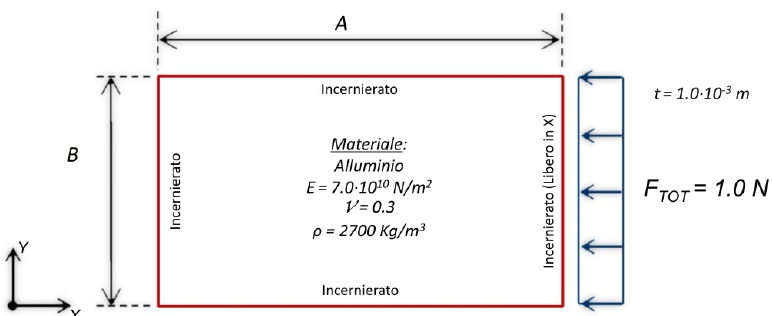
\includegraphics[scale=0.4]{Immagini/piastra.jpg}
	\caption{Piastra caricata di punta}
\end{figure}\\
In particolare si vogliono determinare, mediante solutore FEM (SOL 105), il carico e la deformata critica della piastra al variare della lunghezza A del lato lungo x, ovvero:\\
\begin{center}
	\begin{tabular}{c c c c}
		\hline	
		Caso 1 & $A=1 m$ & $B=1 m$ & $\rho=1$\\
		\hline
        Caso 2 &$A=2 m$ & $B=1 m$ & $\rho=2$\\
        \hline
		Caso 3 &$A=5 m$ & $B=1 m$ & $\rho=5$\\
		\hline
		Caso 4 &$A=.5 m$ & $B=1 m$ & $\rho=.5$\\
		\hline
		
	\end{tabular}
\end{center}
Dalla teoria analitica delle piastre sottili a comportamento flessionale,per la piastra incernierata sui lati, con il lato caricato libero di traslare in direzione x si ha:\\ \\
\textbullet \quad $N_{Cr}(m)=\dfrac{D \pi^2}{b^2}[\dfrac{m}{\rho}+\dfrac{\rho}{m}]^2$\quad $[N/m]$\\ \\
ovvero:\\\\
\textbullet \quad $N_{Cr}(m)=\dfrac{D \pi^2}{b^2}\cdot K$\quad $[N/m]$ \quad \quad\quad \quad \quad \quad\quad \quad
con $K=[\dfrac{m}{\rho}+\dfrac{\rho}{m}]$ \\\\
con autofunzioni, che corrisponder\'a alla deformata critica, pari a:\\\\
\textbullet \quad $\phi_{m n}(x,y)=\sin(\dfrac{m\pi x}{a})\sin(\dfrac{\pi y}{b}) $\\ \\
Notiamo come fissato B il carico critico $N_{Cr}$ dipenda solo dal paramentro $K$, che viene riportato in figura al variare di $\rho$ \\
\begin{figure}[htbp]
	\centering
	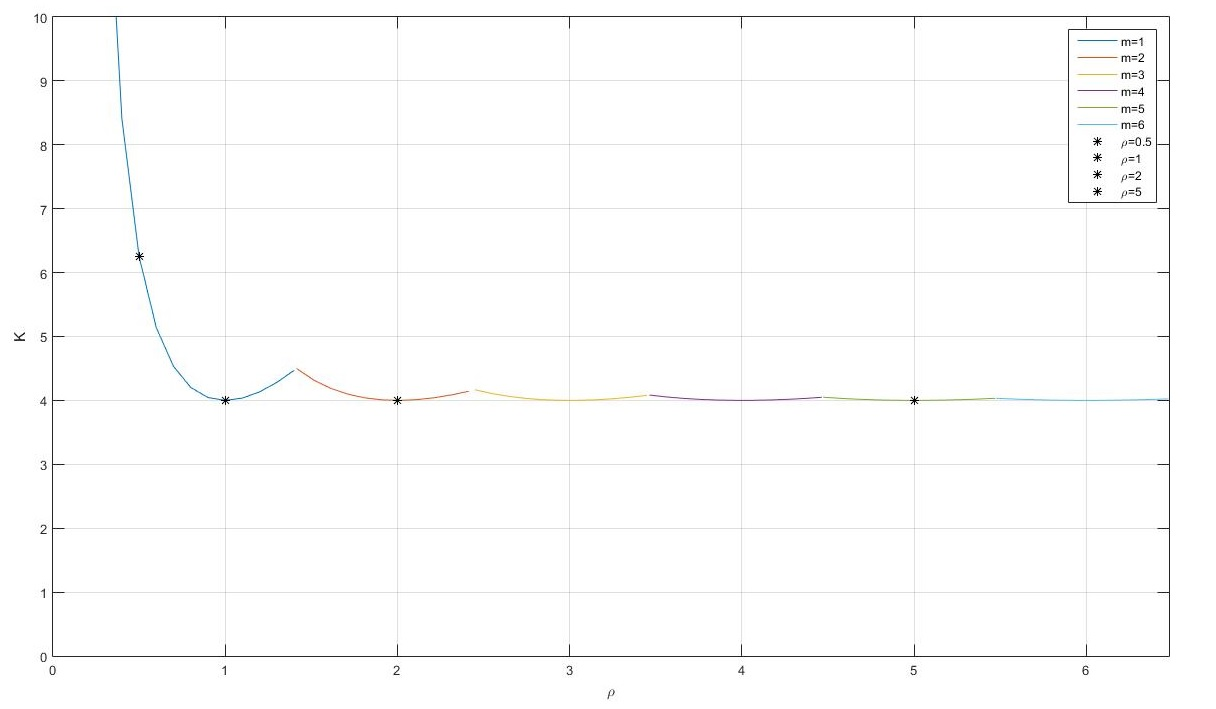
\includegraphics[scale=0.35]{Immagini/K1.jpg}
	\caption{Parametro K al variare di $\rho$}
\end{figure}\\
Si osserva come il parametro $K$ presenti un minimo costante in corrispondenza di $\rho=m$, si noti inoltre che se nel caso in cui il rapporto di rastremazione non sia un numero intero si verifica un innalzamento del parametro K che di fatto corrisponde ad un aumento del carico critico per mandare in instabilit\'a la struttura, innalzamento che \'e sempre meno accentuato al crescere di $m$; infatti a parit\'a di $B$ , il carico critico resta pressoch\'e invariato, ma aumenta il numero di suddivisioni aumenta: la tendenza della deformata sar\'a quella di suddividere in quadrati la piastra.\\
Si noti che nel caso della trave di Eulero la suddivisione non si verifica perch\'e il modello non considera l'effetto irrigidente delle fibre trasversali.\\
Un'altra osservazione degna di nota \'e il caso il cui $\rho<<1$, in questo caso la soluzione si avvicina alla soluzione ottenuta per la trave di Eulero, l'effetto irrigidente delle fibre trasversali viene meno.\\
Si riportano in tabella i valori ottenuti del carico critico dei 4 casi analizzati e il valore di $m$ corrispondente alla deformata critica.\\
\begin{center}
	\begin{tabular}{c c c c}
		\hline	
		Caso 1 & $\rho=1$ & $N_{Cr}=253.07 N $ & $m=1$\\
		\hline
		Caso 2 &$\rho=2 $ & $N_{Cr}=253.07 N $ & $m=2$\\
		\hline
		Caso 3 &$\rho=5 $ & $N_{Cr}=253.07 N $ & $m=5$\\
		\hline
		Caso 4 &$\rho=.5$ & $N_{Cr}=395.42 N$ & $m=1$\\
		\hline
		
	\end{tabular}
\end{center}
Infine sono stati calcolati i carichi critici e deformate critiche con un codice agli elementi finiti, dopo aver opportunamente discretizzato le strutture ,con degli elementi di tipo SHELL, come segue :\\
\begin{center}
	\begin{tabular}{c c c }
		\hline	
		Caso 1 & $A=1 m$ (10 elementi) & $B=1 m$ (10 elementi) \\
		\hline
		Caso 2 &$A=2 m$ (20 elementi)& $B=1 m$ (10 elementi) \\
		\hline
		Caso 3 &$A=5 m$ (50 elementi)& $B=1 m$ (10 elementi) \\
		\hline
		Caso 4 &$A=.5 m$ (10 elementi) & $B=1 m$ (10 elementi) \\
		\hline
		
	\end{tabular}
\end{center}
Ponendo come condizioni al contorno una cerniera lungo il lato x=0, dei carrelli lungo i lati x=A, y=0, y=B lasciando per\'o sempre libera la traslazione lungo y.\\ Infine, per evitare possibili moti di traslazione rigida ma non compromettendo la precisione della soluzione, si \'e vincolata la piastra lungo la mezzeria in modo da non farla traslare lungo y (i lati agli estremi sono liberi di spostarsi e infatti si spostano in modo uguale e contrario essendo la mezzeria un asse di simmetria). Quest'ultimo vincolo \'e necessario per evitare problemi numerici.\\
Inoltre di volta in volta la struttura \'e stata caricata,lungo il lato y=B, con un carico complessivo pari a $\overline{N}=1 N$: applicando delle forze concentrate di intensit\'a pari a $F=\dfrac{1}{N_{nodi}}$ $N$ su ognuno dei nodi del lato caricato y=B.\\
Si riportano i risultati in termini di moltiplicatore di carico:\\
\begin{center}
	\begin{tabular}{c c c }
		\hline	
		Caso 1 & $\rho=1$ & $N_{CrFEM}=252.92 N $ \\
		\hline
		Caso 2 &$\rho=2 $ & $N_{CrFEM}=252.93 N $ \\
		\hline
		Caso 3 &$\rho=5 $ & $N_{CrFEM}=253.71 N $ \\
		\hline
		Caso 4 &$\rho=.5$ & $N_{CrFEM}=396.19 N$ \\
		\hline
		
	\end{tabular}
\end{center}
Si noti come i risultati sono in forte accordo con quelli ottenuti per via analitica.\\
Vengono riportate le deformate critiche per completezza.\\
\begin{figure}[htbp]
	\subfloat[][\emph{Deformata critica, piastra $\rho=0.5$}.]
	{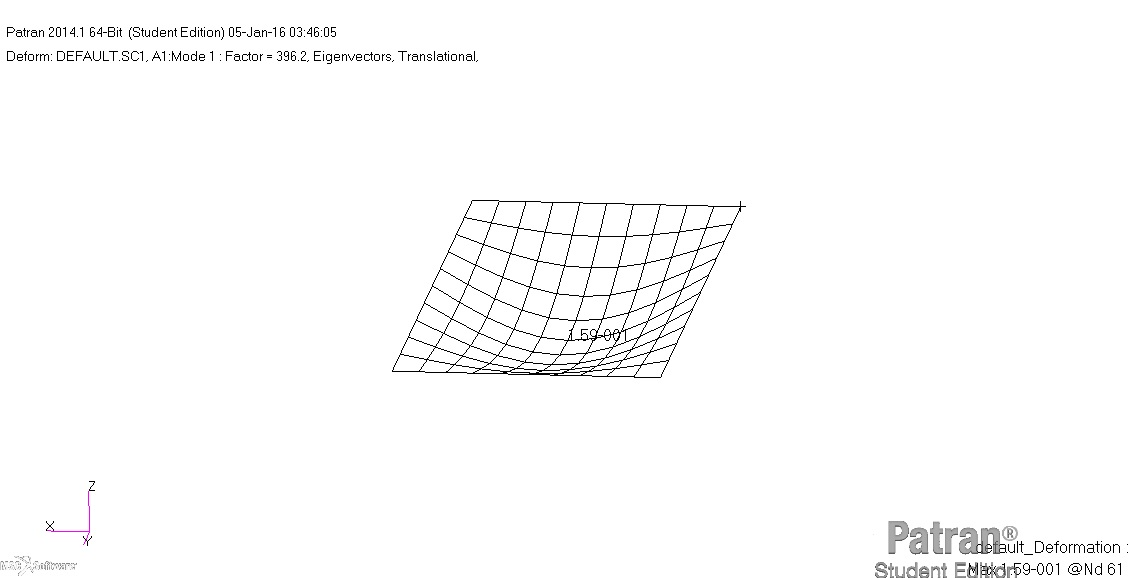
\includegraphics[width=.55\textwidth]{Immagini/Piastraa05b1.jpg}} \quad
	\subfloat[][\emph{Deformata critica, piastra $\rho=1$}.]
	{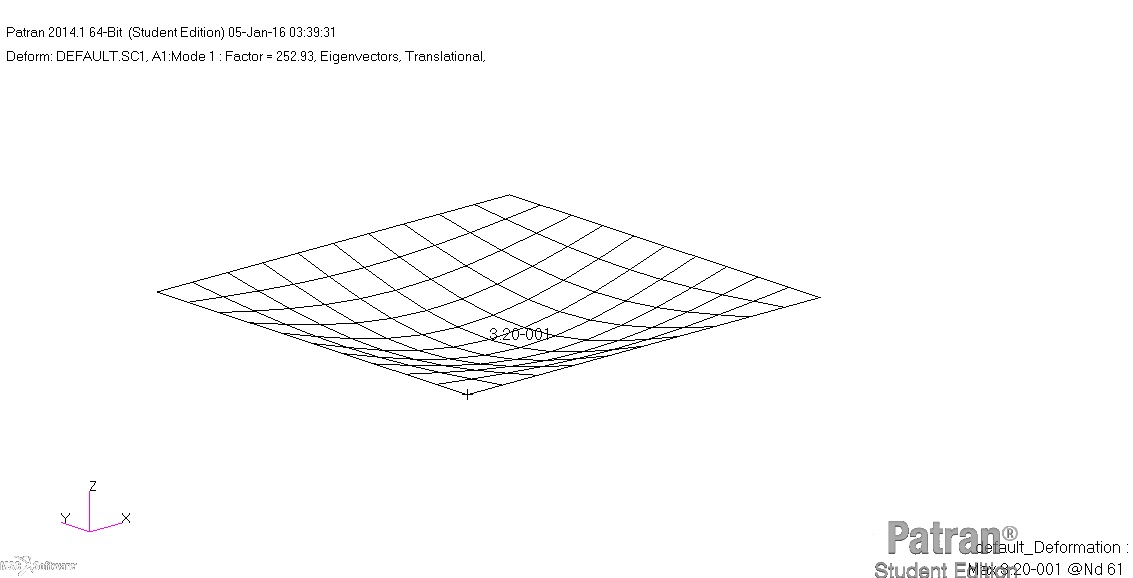
\includegraphics[width=.55\textwidth]{Immagini/Piastraa1b1.jpg}} 
	\label{fig:subfig}
\end{figure}
\begin{figure}[htpb]
	\subfloat[][\emph{Deformata critica, piastra $\rho=2$}.]
	{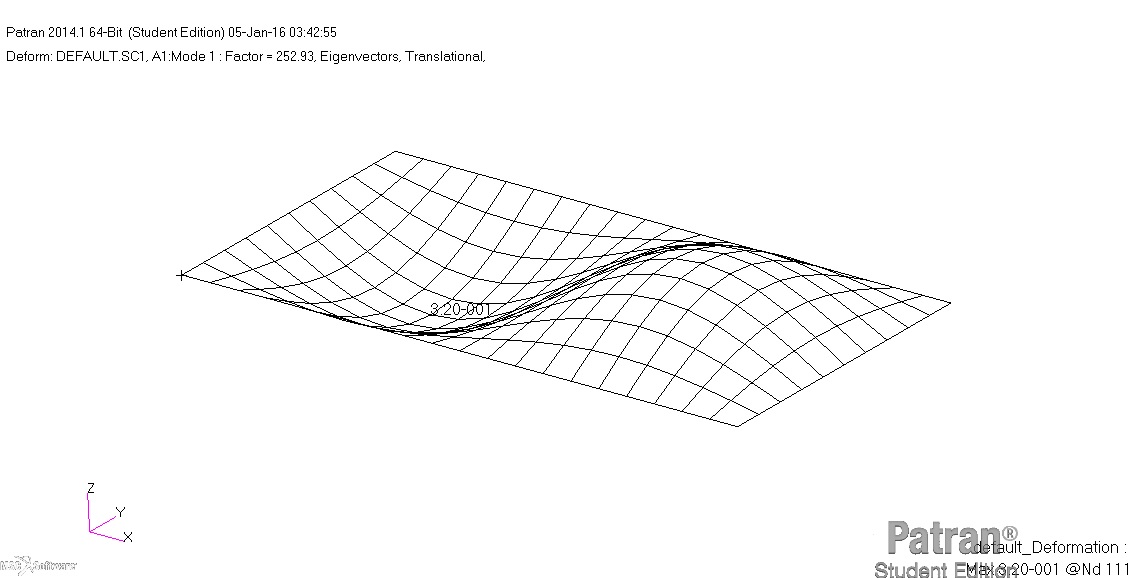
\includegraphics[width=.55\textwidth]{Immagini/Piastraa2b1.jpg}} \quad
	\subfloat[][\emph{Deformata critica, piastra $\rho=5$}.]
	{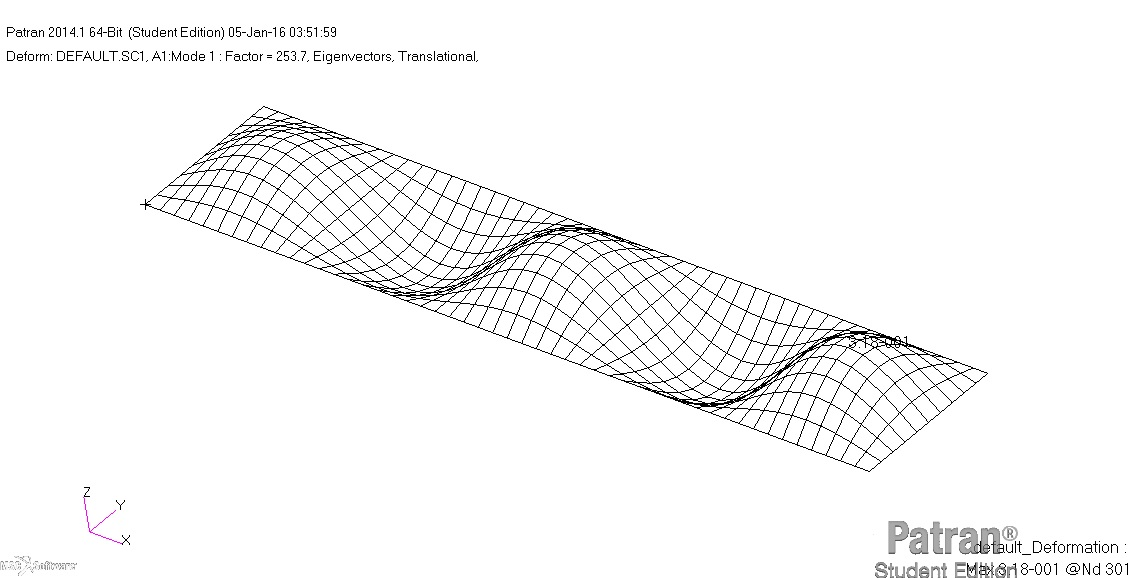
\includegraphics[width=.55\textwidth]{Immagini/Piastraa5b1.jpg}} 
	\label{fig:subfig}
\end{figure}
\newpage
\section{Cilindro caricato in punta}
Il secondo ed ultimo caso trattato \'e quello di un cilindro, in parete sottile, costituito da una lega leggera (alluminio) di spesspre $t=2 mm$ incernierato alle due estremit\'a, e caricato su una delle estremit\'a da una forza di compressione uniformemente $\overline{N}$ ditribuita sul bordo, cosi come mostrato in figura.\\
\begin{figure}[htbp]
	\centering
	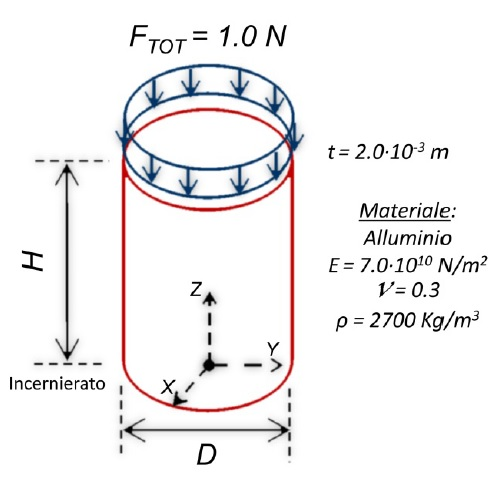
\includegraphics[scale=0.4]{Immagini/Cilindro.jpg}
	\caption{Cilindro in parete sottile caricato in punta}
\end{figure}\\
In particolare si vogliono determinare, mediante solutore FEM (SOL 105), il carico e la deformata critica del cilindro al variare della lunghezza H del cilindro, ovvero:\\
\begin{center}
	\begin{tabular}{c c c}
		\hline	
		Caso 1 & $D=1 m$ & $H=.5 m$ \\
		\hline
		Caso 2 &$D=1 m$ & $H=1 m$ \\
		\hline
		Caso 3 &$D=1 m$ & $H=5 m$ \\
		\hline
		
	\end{tabular}
\end{center}
Dalla teoria analitica dei gusci cilindrici a comportamento flessionale, per il cilindro incernierato su entrambe le estremit\'a e con quella caricata libera di traslare in direzione z del cilindro si ha:\\ \\
\textbullet \quad $N_{Cr}(m)=D(\dfrac{m \pi}{l})^2+\dfrac{Et}{r^2}(\dfrac{l}{m\pi})^2$ \quad $[N/m]$\quad \quad \quad con $r=$raggio del cilindro \\\\ ovvero in termini di $\sigma_{Cr}$:\\\\
\textbullet \quad $\sigma_{Cr}=D(\dfrac{\alpha^2}{t}+\dfrac{E}{Dr^2}\dfrac{1}{\alpha^2})$\quad\quad\quad\quad\quad\quad\quad\quad\quad\quad\quad\quad
con $\alpha^2=(\dfrac{m\pi}{l})^2$ \\\\
con autofunzioni, che corrisponder\'a alla deformata critica, pari a:\\
\textbullet \quad $\phi_{m}(x)=\sin(\dfrac{m\pi x}{l}) $\\ \\
La condizione minimizzante il carico critico la trovo imponendo:\\\\
\textbullet \quad $\dfrac{\partial\sigma}{\partial\alpha}$\\\\
trovando:\\\\
\textbullet \quad $\alpha_{min}^4=\dfrac{Et}{Dr^2}$\\\\
ovvero tenendo presente la definizione di $\alpha$ si ha:\\\\
\textbullet \quad $m=\dfrac{l}{\pi}\sqrt[4]{\dfrac{Et}{Dr^2}}$\\\\
 facendo attenzione al fatto che $m$ \'e una variabile di natura discreta, quindi una volta stimato $m$ si deve calcolare il valore del carico critico in corrispondenza di $m$ ma anche di $m-1$ e $m+1$ cio\'e in corrispondenza del valore precedente e successivo di $m$ rispettivamente.\\
 Svolgendo i calcoli tenendo a mente le considerazioni precedenti si giunge ai seguenti risultati:\\
\begin{center}
	\begin{tabular}{c c c c c }
		\hline	
		Caso 1 & $D=1 m$ $H=.5 m$& $m=9$ & $N_{Cr}=339.11$ $[kN/m]$&$\sigma_{Cr}=169.56$ $MPa$ \\
		\hline
		Caso 2 &$D=1 m$ $H=1 m$ &$m=18$ &$N_{Cr}=339.11$ $[kN/m]$&$\sigma_{Cr}=169.56$ $MPa$\\
		\hline
		Caso 3 &$D=1 m$ $H=5 m$&$m=92$ &$N_{Cr}=338.95$ $[kN/m]$&$\sigma_{Cr}=169.47$ $MPa$\\
		\hline
		
	\end{tabular}
\end{center}
Infine sono stati calcolati i carichi critici e deformate critiche con un codice agli elementi finiti, dopo aver opportunamente discretizzato le strutture, con degli elementi di tipo SHELL, come segue :\\
\begin{center}
	\begin{tabular}{c c c }
		\hline	
		Caso 1 & $D=1 m$ (40 elementi) & $H=.5 m$ (20 elementi) \\
		\hline
		Caso 2 &$D=1 m$ (40 elementi)& $H=1 m$ (40 elementi) \\
		\hline
		Caso 3 &$D=1 m$ (40 elementi)& $H=5 m$ (100 elementi) \\
		\hline
		
	\end{tabular}
\end{center}
Dopo aver definito un sistema di riferimento cilindrico ($r$ $\theta$ $z$) si sono poste le seguenti condizioni al contorno:\\ la base inferiore \'e incernierata mentre la base superiore, quella su cui \'e applicato il carico, � libera di traslare solo nella direzione parallela all'asse del cilindro ed � libera di ruotare solo intorno alla direzione $\theta$ tangente alla base cilindro.\\
Ovvero per l'estremit\'a superiore di applicazione del carico si sono vincolati i gradi di libert\'a (T1 T2 R1 R3) mentre su quella inferiore i gradi di libert\'a (T1 T2 T3 R1 R3), sempre nel sistema di riferimento cilindrico.\\
Inoltre per ogni caso si \'e applicato un carico di compressione sulla base superiore, libera di scorrere, di intensit\'a pari a $\overline{N}=1N$; nei primi due casi \'e stata applicata un'unica forza di $\overline{N}=1 N$ su un nodo centrale aggiunto sulla base superiore e poi grazie all' utilizzo degli elementi RBE3 la si \'e distribuita in modo uniforme sui i nodi di interesse (indipendentemente dal loro numero), vincolando questo nuovo nodo con quelli della base superiore.\\
Nell'ultimo caso invece si sono applicate su ognuno dei 40 nodi dell'estremit\'a superiore, delle forze concentrate , di compressione, di intensit\'a pari a $F=0.025$ $N$.\\
Si riportano i risultati ottenuti in termini di tensioni e carico critico.


\begin{center}
	\begin{tabular}{ c c c c }
		\hline	
		 $H=.5 m$&$N_{CrFEM}=1074.32$ $[kN]$ & $N_{CrFEM}=341.86$ $[kN/m]$&$\sigma_{CrFEM}=170.95$ $MPa$ \\
		\hline
		$H=1 m$ &$N_{CrFEM}=1066.18$ $[kN]$ &$N_{CrFEM}=339.37$ $[kN/m]$&$\sigma_{CrFEM}=169.68$ $MPa$\\
		\hline
	 $H=5 m$&$N_{CrFEM}=1066.24$ $[kN]$ &$N_{CrFEM}=339.24$ $[kN/m]$&$\sigma_{CrFEM}=169.70$ $MPa$\\
		\hline
		
	\end{tabular}
\end{center}
I risultati sono in forte accordo con quelli ottenuti per via analitica.\\ Tuttavia la teoria analitica prevede una diminuzione del carico critico al crescere di $H$, mentre i risultati ottenuti tramite solutore FEM mostrano un comportamento pressoch\'e costante nel passaggio da $H=1$ e $H=5$, questo pu\'o essere spiegato dal fatto che la versione studenti di MSC Nastran non permette mesh abbastanza fitte da poter seguire la geometria della deformata critica (m=92).\\
Per completezza si riportano le deformate critiche ottenute tramite solutore FEM.
\newpage
\begin{figure}[htbp]
	\subfloat[][\emph{Deformata critica, cilindro $H=0.5 m$}.]
	{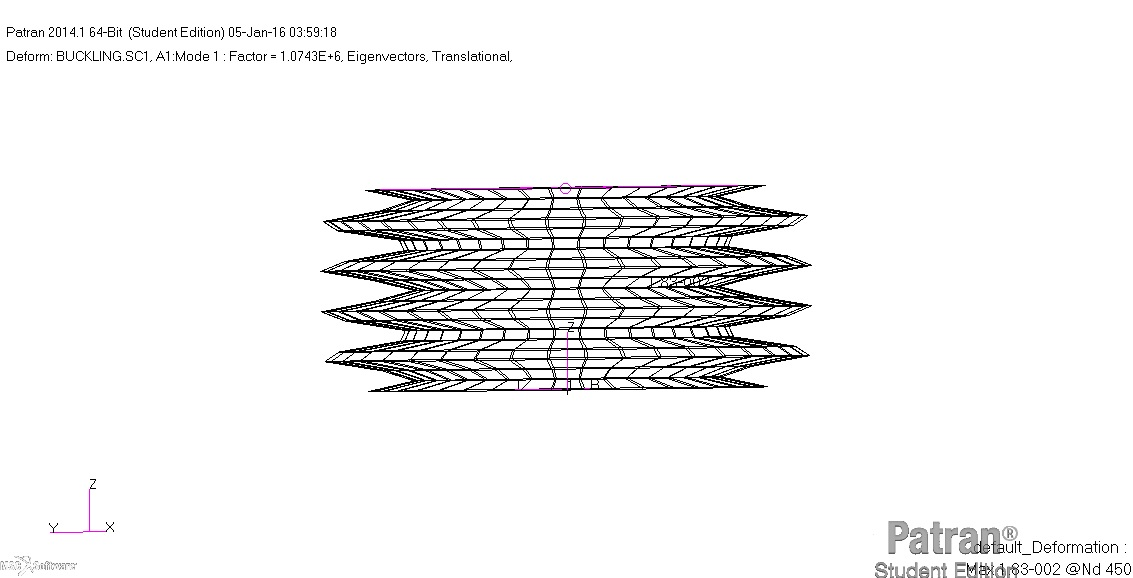
\includegraphics[width=.55\textwidth]{Immagini/Cilindrod1h05.jpg}} \quad
	\subfloat[][\emph{Deformata critica, piastra $H=1m$}.]
	{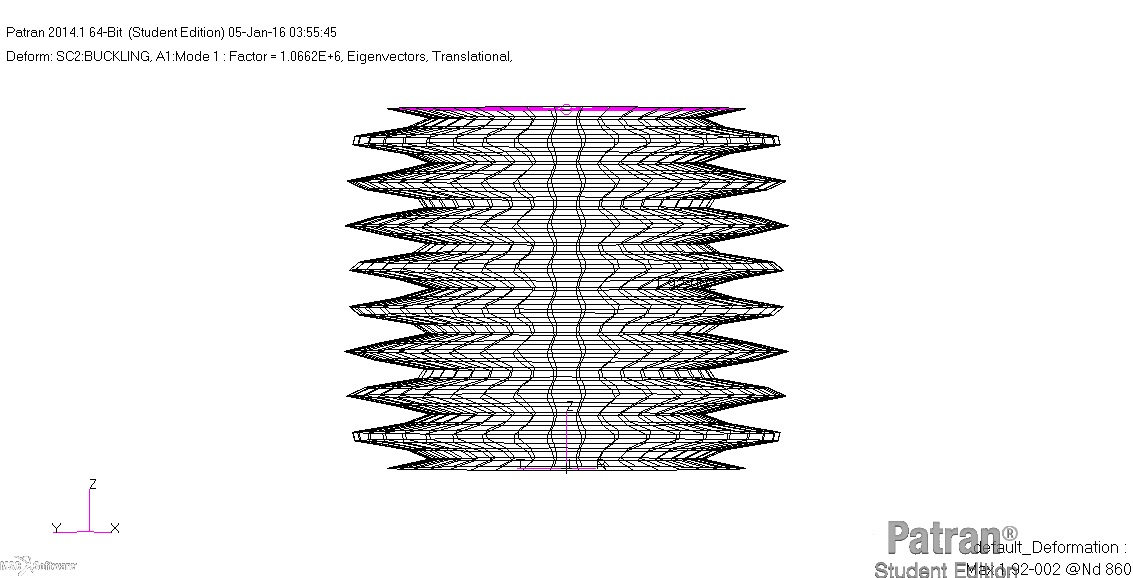
\includegraphics[width=.55\textwidth]{Immagini/Cilindrod1h1.jpg}} 
	\label{fig:subfig}
\end{figure}
\begin{figure}[htbp]
	\centering
	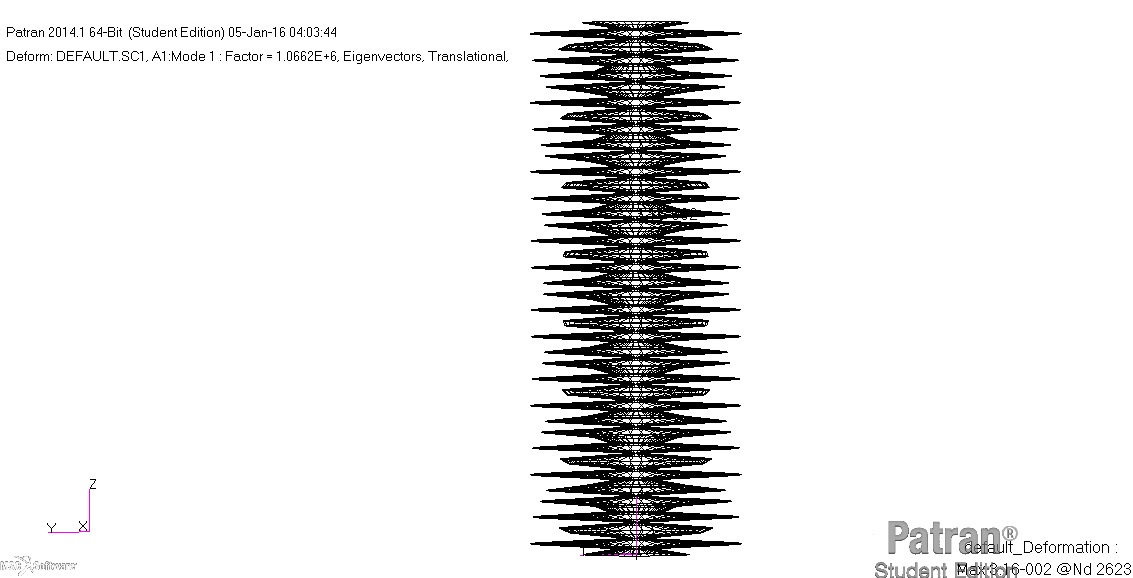
\includegraphics[scale=0.28]{Immagini/Cilindrod1h5.jpg}
	\caption{Deformata critica, cilindro $H=5m$}
\end{figure}













\end{document}